Traditionally, people consider semantic parsing and information extraction approaches to knowledge base question answering \cite{yao2014freebase}.
The former focuses on question understanding and attempts to parse the sentences into some kind of semantic representation, \eg logical forms \cite{Berant:EMNLP13,berant2014semantic,berant2015imitation}.
Information extracting approaches \cite{ACCU:2015,yih2015semantic,yao2014information} are based on identifying question topical entities, exploring the neighborhood of these entities in a KB using a set of query template and ranking these candidates.
Theoretically, semantic parsing approaches are capable of generating complex queries, which are hard to cover with a reasonable set of templates.
But in practice, answers to most of the questions lie within two edges in a KB, and that is why information extraction approaches turn out to be very effective.

One of the most popular benchmark datasets for knowledge base question answering is WebQuestions \cite{Berant:EMNLP13}, which has attracted a lot of attention recently and as a result the performance increased from 0.357 \cite{Berant:EMNLP13} to 0.525 \cite{yih2015semantic} in average F1 over test questions.
The dataset is based on Freebase, which has been recently shut down\footnote{https://goo.gl/SZC3tg}.
The shutdown of Freebase means that it will no longer be extended, but all the data will be available and it will be merged with WikiData\footnote{https://www.wikidata.org/}.
Therefore, future datasets should probably use different reference KB, but there is no problem in using Freebase for experiments on existing benchmarks, such as WebQuestions.
We should also stress, that the proposed approach isn't tied to Freebase and can be applied for question answering over dbPedia, WikiData or other knowledge bases.

The focus of this work is on the fusion between structured data in the KB and unstructured text data.
Therefore, we chose to extend an existing KBQA system: Accu \cite{ACCU:2015}.
It follows an information extraction approach to KBQA and achieves one of the highest scores among publicly available systems.
However, our approach can be incorporated into other systems as well.

We will first describe an information extraction approach to KBQA in more detail using Accu - our baseline system - as an example, and Section \ref{section:method} will present our system Text2KB, which extends the baseline by incorporating external text-based data on various stages of the question answering process.

\begin{figure*}[!ht]
\centering
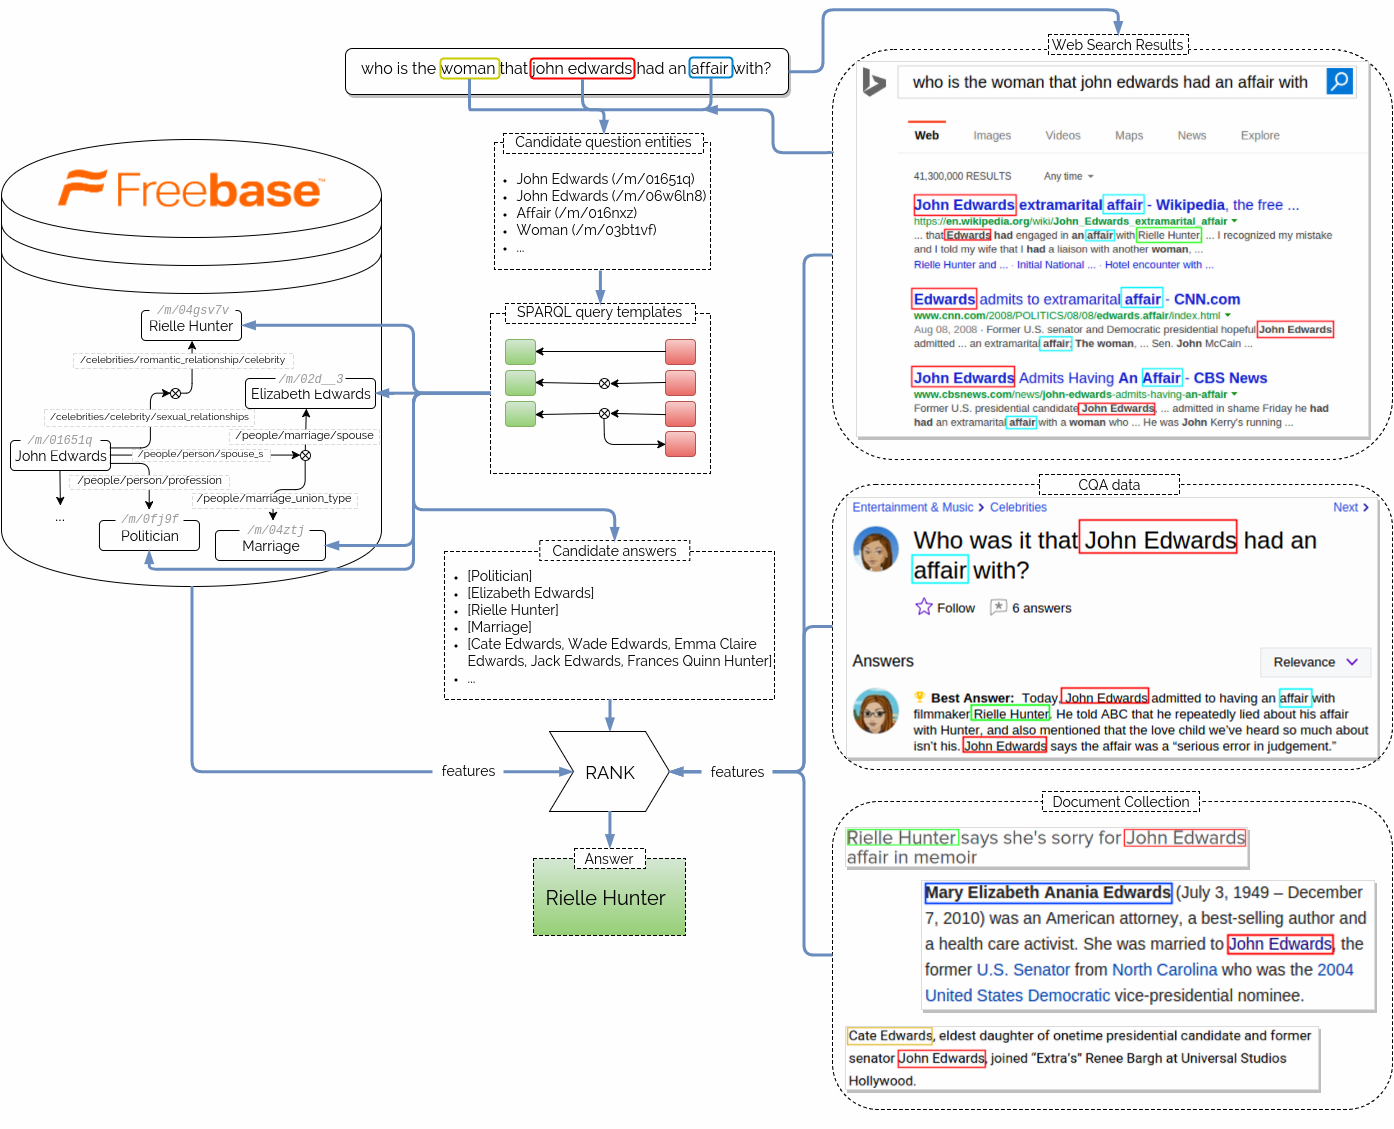
\includegraphics[width=\textwidth]{img/Text2KB_model}
\caption{The architecture of our Text2KB Question Answering system}
\label{fig:model}
\end{figure*}


\subsection{Our baseline system}

Let's consider a question \textit{``who is the woman that john edwards had an affair with?''}.
First, the system identifies a set of possible question entities.
In our example, entity \texttt{John Edwards} with Freebase mid \texttt{/m/01651q} is the main question entity.
However, Freebase contains millions of entities and it's often hard to identify the topical ones (\eg entities \texttt{Woman} and \texttt{Affair} are also present in Freebase) or to disambiguate and choose between \texttt{John Edwards} a politician (\texttt{/m/01641q}), \texttt{John Edwards} an American sports car racing driver (\texttt{/m/06zs089}) and other people with the same name.
There is even an entity with the name ``\texttt{had an affair with}''\footnote{http://www.freebase.com/m/0c0n01x}.
Accu considers all spans of terms under certain conditions on POS tags and use a dictionary of names, aliases and anchor tests \cite{SPITKOVSKY12.266} to map phrases to potential entities.
Most recent systems, including Accu, don't disambiguate entities at this stage and keep a set of candidates along with some information about entity popularity and mention scores.

On the next stage answer SPARQL query candidates are generated by exploring the neighborhood of the question topical entities usign a predefined set of query templates.
Each query template has an entity, predicate and answer entity placeholders.
Majority of the answers in WebQuestions dataset can be covered by just 3 templates (q\_entity - question entity, a\_entity - answer entity, cvt\_node - Freebase mediator node, which represent tuples with more than 2 arguments):

\begin{lstlisting}[frame=single]
SELECT DISTINCT ?a_entity {
   <q_entity> <predicate> ?a_entity .
}
\end{lstlisting}

\begin{lstlisting}[frame=single]
SELECT DISTINCT ?a_entity {
   <q_entity> <predicate_1> ?cvt_node .
   ?cvt_node <predicate_2> ?a_entity .
}
\end{lstlisting}

\begin{lstlisting}[frame=single]
SELECT DISTINCT ?a_entity {
   <q_entity_1> <predicate_1> ?cvt_node .
   ?cvt_node <predicate_2> <q_entity_2> .
   ?cvt_node <predicate_3> ?a_entity .
}
\end{lstlisting}

The first template retrieves a set of entities that are directly connected to the given question entity via a certain predicate.
The second template accounts for the presence of a mediator node, that groups together arguments of a multi-argument relation.
And the last template looks for cases, when multi-argument relations also mentions another question entity, \eg \texttt{Captain Kirk} and \texttt{Star Trek} for the question \textit{``who played captain kirk in star trek movie?''}.

%\begin{enumerate}
%\item \texttt{$[$q\_entity$]$ $\rightarrow$ $[$predicate$]$ $\rightarrow$ $[$a\_entity$]$}
%\item \texttt{$[$q\_entity$]$ $\rightarrow$ $[$predicate$_1]$ $\rightarrow$ $[$cvt\_entity$]$\\
%$[$cvt\_entity$]$ $\rightarrow$ $[$predicate$_2]$ $\rightarrow$ $[$a\_entity$]$}
%\item \texttt{$[$qentity$_1]$ $\rightarrow$ $[$predicate$_1]$ $\rightarrow$ $[$cvt\_entity$]$\\
%$[$cvt\_entity$]$ $\rightarrow$ $[$predicate$_2]$ $\rightarrow$ $[$q\_entity$_2]$\\
%$[$cvt\_entity$]$ $\rightarrow$ $[$predicate$_3]$ $\rightarrow$ $[$a\_entity$]$}
%\end{enumerate}

Finally, each query candidate is represented with a set of features, that include information about the popularity of question entities (mention frequency), entity linking mention score, size of the answer entity list, how many tokens from the questions match to entities used in the candidate, how many tokens match predicates via exact match by its name or using a dictionary of terms learned for each predicate using distant supervision from a large text corpus, \eg ClueWeb\footnote{http://www.lemurproject.org/clueweb12/}, and some other.
One of the most useful features is a score from a logistic regression model, that predicts whether a predicate answers the question represented as a set of uni- and bigrams.
The full list of features can be found in the original paper \cite{ACCU:2015}.

The final stage of the question answering process is query candidate filtering and ranking.
To rank candidates are sorted in such a way, that pairs of candidates are compared using trained random forest model.

\subsection{Baseline system extensions}
Preliminary analysis of the system suggested a couple of directions for improvement, that do not require an external data sources.
First, we noticed that since the system doesn't really use information about answer entity Freebase types, in many cases it returns an answer that is type incompatible with the question: \eg state instead of county \etc
Similarly to how relations are scored in Accu, we decided to train a model to predict how likely a certain notable entity type is the answer of a question, represented as a set of uni- and bigrams.
The score of this model is used as a feature for candidate ranking.

A second introduces a new date range query template.
\begin{lstlisting}[frame=single]
SELECT DISTINCT ?a_entity {
   <q_entity_1> <predicate_1> ?cvt_node .
   ?cvt_node <from_predicate> ?date_from .
   ?cvt_node <to_predicate> ?date_to .
   ?cvt_node <predicate_2> ?a_entity .
   FILTER (
   	<question_date> >= ?date_from AND
   	<question_date> <= ?date_to
   )
}
\end{lstlisting}

This template helps to solve the cases like \textit{``what team did david beckham play for in 2011?''}, where we need to look at the ranges of dates of figure out in which range does the specified date falls.
We also experimented with additional template, that filters out lists by entity notable types.

